\documentclass[twoside]{wiss}
%
%
% 問題を作るのが面倒だから、シードや回答を変えて運用するのがいい
%
% 最近の人はなんでもtweetするから大変
% 不倫とかぐらいしかないかも
% 「該当なし」を用意するべき
%
% 応用例
%   家族でパスワードをシェア
%   WiFiのパスワードを学会でシェアするとか
%   ライセンスキーとかすべて
%   暗号化のキー?
%
% 利点は本文を見ればなんとなくわかるようになっていればいい
%  忘れないこと
%  テキストとして管理すればいいこと
%  様々な運用形態があること

% 小学校のときの怪我とか悪事とかが良い問題になるのではないか
% 旅行のときの経験とか

%
% パスワードのハッシュが流出したら総当たりでわかってしまうかも
% レインボーテーブルなどを使うより簡単にわかる
% その場合でもソルトが使われていれば大丈夫
% つまりパスワードを使った認証システムがちゃんとするべきだということ

% なんでもしゃべってしまう人はそれ以外のパスワードとあわせ技にするといいかも

%\usepackage{ascmac}

\usepackage{graphicx}
\usepackage{here} % [H]とするとその場所に配置されるらしい

\long\def\EP{\textsf{EpisoPass}}
\long\def\PW{パスワード}
\long\def\SS{シード文字列}
\long\def\EM{エピソード記憶}
\long\def\SQ{秘密の質問}

\journalhead{{\EP}: Password Management based on Episodic Memories}

\begin{document}

\title{{\EP}: {\EM}にもとづく{\PW}管理}
%\etitle{{\EP}: The Ultimate Passwords Management System}
\etitle{{\EP}: Password Management based on Episodic Memories}

\author{増井俊之\affil{Toshiyuki Masui, 慶應義塾大学 環境情報学部}}

\begin{abstract}
忘れることがない{\EM}にもとづく{\SQ}を使って強力な{\PW}を生成/管理するシステム「\textsf{\EP}」を提案する。
{\EP}は、ユーザが作成した{\SQ}への回答にもとづいて{\SS}を換字することによって{\PW}を生成する。
{\SS}や回答のバリエーションにより異なる{\PW}が生成されるので様々なサービスに対して異なる{\PW}を生成できることに加え、
{\SS}を逆計算することにより既存の{\PW}の管理もできる。
適切な運用により、{\PW}に関連するあらゆる情報を秘密にすることなく
強力な{\PW}の生成/管理が可能である。
\end{abstract}

% We introduce a password generation/management system called EpisoPass,
% which converts a seed string into a password using the user's
% episodic memories represented as a set of questions and answers
% which can be solved only by the user.
% Using EpisoPass with well-defined questions and answers,
% a user can always retrieve various passwords without worrying about
% remembering secret information.

\maketitle

\section{はじめに}

個人認証のために{\PW}が現在広く利用されている。
{\PW}認証には多くの問題があることが知られているが\cite{増井_ユニマガ}、
今後も長期にわたって利用され続けると予想されるため\cite{Herley:2009:PSS:1601990.1602010}、
問題点を認識しつつ
適切に運用するための工夫が必要である。

{\PW}の長期的記憶が難しいことは{\PW}認証の大きな問題点のひとつである。
安全に運用するためには{\PW}はランダムで長い文字列であることが望ましいが、
そのようなものを頭の中に記憶しておくことは難しい。
また複数のサービスを利用する場合、
サービスごとに異なる{\PW}を利用することが望ましいが、
すべての{\PW}を記憶しておくことはほとんど不可能である。
%
Flor\^{e}ncioの2007年の大規模な調査によれば、
ユーザは平均25個のサイトで6.5個の{\PW}を利用しており、
3ヶ月間にユーザの4.28\%が{\PW}を忘れていた\cite{Florencio:2007:LSW:1242572.1242661}。
また2011年の野村総研の調査によれば、
一般的なユーザが{\PW}認証を行なうサイトは平均19.4個で、
利用している{\PW}は平均3.1個であった\cite{野村総研}。
多数の{\PW}を記憶することが困難であるため、
多くのユーザが同じ{\PW}を複数サイトで使い回しているのだと思われる。

異なる{\PW}をすべて記憶することは不可能なのでどこかに記録しておく必要があるが、
{\PW}文字列をそのまま記録するのは危険なので、
複数の{\PW}を秘密情報として扱うための{\PW}管理システムが利用されている。
{\PW}管理システムは
ひとつの「マスター{\PW}」を利用して他のすべての{\PW}を管理するもので、
暗号化されたデータベースに{\PW}を格納するもの%
\cite{OnePassword}%
\cite{Dashlane}%
\cite{ミルパス}%
\cite{LastPass}%
\cite{KeyPass}%
\cite{NortonIDSafe}%
\cite{IDManager}%
が多いが、サービス名をもとにマスター{\PW}を変換することによって
複数の{\PW}を生成するシステム\cite{SuperGenPass}もある。
% 前者はデータベースを解読される危険があるのに対し、
% 後者は{\PW}本体をどこにも保存していないためより安全であるが、
両者ともにマスター{\PW}の記憶は必須であり、
マスター{\PW}を盗まれたり忘れたりする危険がある。
% {\PW}を毎日使わない人なら忘れてしまう可能性は高い。

一般にユーザは{\PW}を忘れがちであるため、
多くのサービスにおいて{\PW}を復元したり初期化したりする手段が用意されている。
ユーザが{\SQ}に対する答を登録し、
質問に正しく回答することによって{\PW}を復元したりリセットできるサービスは多いし、
{\SQ}に答えることによって
{\PW}管理システムのマスター{\PW}を復元するシステム\cite{平野亮:2011-11-07}も提案されている。

新しく覚えた情報や新しく考えた情報はどうしても忘れてしまう可能性があるので、
新しく作成した{\PW}文字列を記憶して認証に利用することは本質的に無理がある。
一方、既知で忘れることがない{\EM}を{\SQ}として
認証のために直接利用することができれば、
認証に必要な情報を忘れてしまうことがないはずである。
多くの画像認証システム\cite{Biddle:2012:GPL:2333112.2333114}\cite{小池英樹:2006-05-15}\cite{GraphicalPasswords}は
{\SQ}に対して適切な操作を行なうことによって認証を行なっているため
{\PW}のようなものを記憶する必要がない。
%認証方法を忘れにくいという特長がある。
% {\SQ}が{\PW}と同じぐらい強力であれば、
% それをメインの認証手段にしてしまえばいいことになる。
%
画像認証システムはまだ普及しておらず利用できる環境は限られているが、
忘れない{\EM}を利用した{\SQ}への回答を強力な{\PW}に変換するシステムがあれば、
通常の{\PW}認証を用いた現在の様々なサービス上で、
認証方法を忘れる心配なく安全に認証を行なうことができるようになる。
本論文ではこのようなシステム「{\EP}」について述べる。

\section{{\EP}}

\subsection{{\EP}の原理}

{\EP}は、
ユーザが忘れることがない個人的な{\EM}を文字列に変換することによって
安全な{\PW}を生成するシステムである。
{\PW}文字列は以下の手順で生成される。

\begin{enumerate}
\item {\PW}生成の「種」となる文字列を用意する。
以下ではこれを「{\SS}」と表現する。
\item 忘れることがない個人的な{\EM}にもとづく{\SQ}を複数作成し、
それぞれについてひとつの正答と複数の偽答を用意する。
\item 質問と回答の組にもとづいて{\SS}に換字操作を行なう。
すべてに正しく回答したとき生成される文字列を{\PW}として利用する。
\end{enumerate}

\subsection{{\EP}利用例}

以下に{\EP}の利用例を示す。

\subsubsection{ブラウザでの利用}

筆者がtwitterの{\PW}を生成するために
ブラウザで{\EP}を利用している例を図\ref{web1}に示す\footnote{
  \textsf{http://{\EP}.com/masui}
}。
{\SS}として「\textsf{Twitter123456}」という文字列を指定しており、
4個の{\SQ}に対する回答選択に応じて
「\textsf{Mfveabn574923}」のような{\PW}候補が生成される。
異なる答をを選択すると全く異なる文字列が生成される。
{\SS}の8文字目が数字である場合は{\PW}の8文字目も数字になるなど、
{\SS}の文字種に対応した{\PW}候補が生成される。

最初の{\SQ}は筆者の小学校の同級生に関するもので、
最後の質問は数年前の体験に関するものである。
これらの質問は古い{\EM}にもとづいており、
筆者が将来答を忘れることはほとんど考えられないが、
本人以外がこのような質問に答えることは難しいので
正しい{\PW}を得ることはできない。

\begin{figure}[H]
\centerline{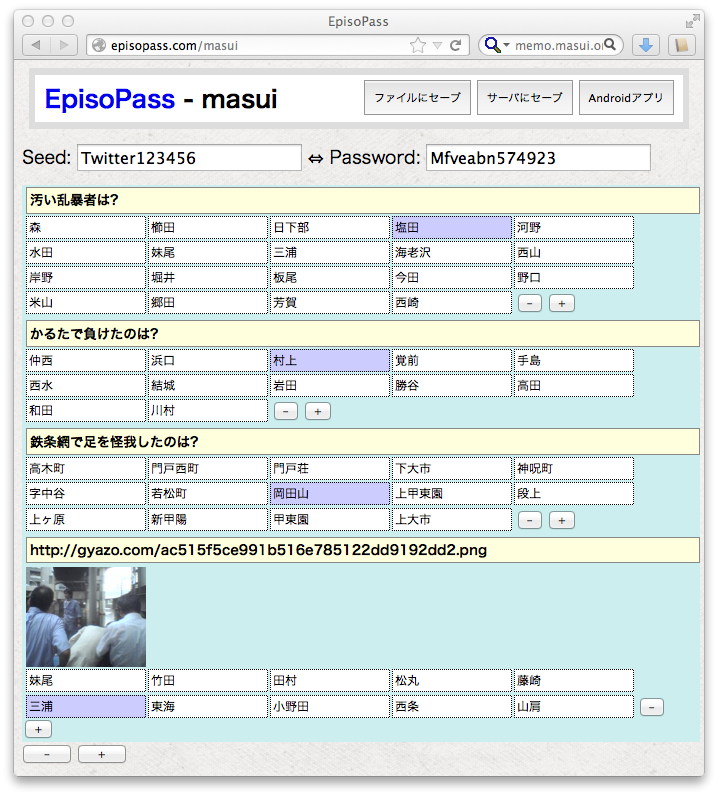
\includegraphics[width=83mm,bb=0 0 718 796]{figures/785ff09b4233804d2ec89c3af71ee5d0.png}}
\caption{ブラウザ上でTwitterの{\PW}を生成.}
\label{web1}
\end{figure}

{\SQ}と答はブラウザで編集でき、
右上の「サーバにセーブ」ボタンを押すことにより{\SS}、秘密の問題、答のリストがサーバにセーブされる。
「ファイルにセーブ」ボタンを押すとJSONデータをパソコンにダウンロードでき、
パソコン上のJSONデータをブラウザにドラッグ\&ドロップするとサーバにアップロードできる。
ユーザはどれが正答かを指定するわけではないので
問題データを見てもユーザの{\PW}はわからない。

{\SS}を「\textsf{Facebook123456}」に変更すると、生成される{\PW}は図\ref{web2}のように変化する。
このように、サービスごとに異なる{\SS}を利用することによって
様々な{\PW}を簡単に生成できる。

\begin{figure}[H]
\centerline{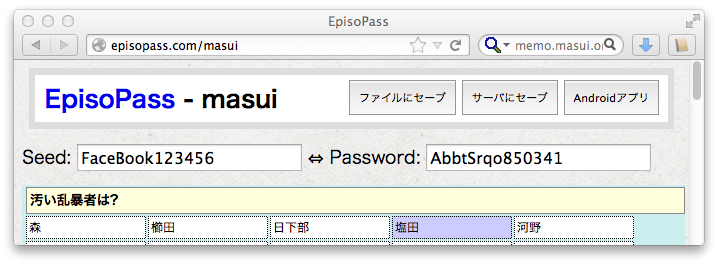
\includegraphics[width=83mm,bb=0 0 718 265]{figures/36c371a13a8250c60fb9c03174382443.png}}
\caption{FaceBookの{\PW}を計算.}
\label{web2}
\end{figure}

{\PW}として大文字/小文字英数字と記号をすべて利用しなければならないサービスの場合は
{\SS}に「\textsf{PassWord123!@\#}」のような文字列を指定すればよい。

\subsubsection{回答選択により{\PW}を切り換え}
\label{pwgen}

サービスごとに{\SS}を変えるのではなく、
図\ref{web3}のように
サービス名に応じて回答を変えることによって異なる{\PW}を作成することも可能である。
{\PW}としての長さや文字種に特種な制約が無いサービスに関してはこの方法が便利である。

\begin{figure}[H]
\centerline{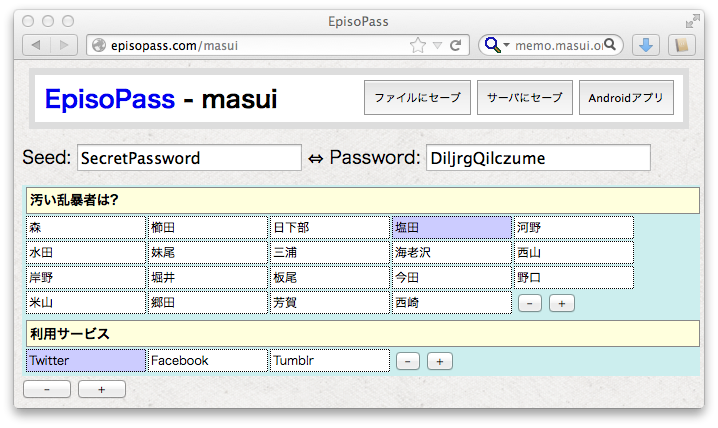
\includegraphics[width=83mm,bb=0 0 718 428]{figures/a9167a6ec6af9c70dd1617e3fc25ec30.png}}
\centerline{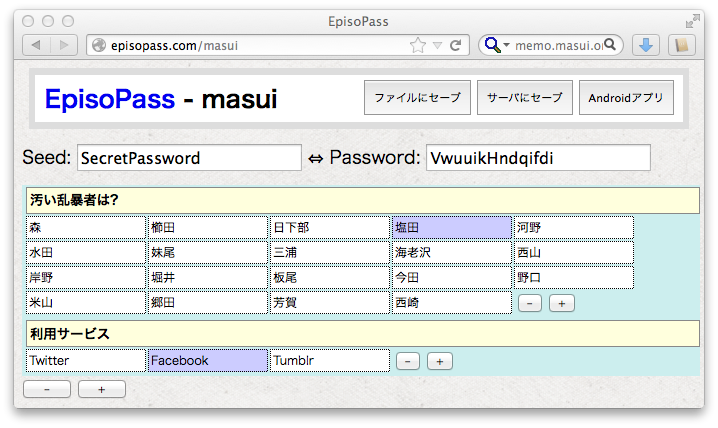
\includegraphics[width=83mm,bb=0 0 718 428]{figures/5b887fabeb8e3319623901fe4a6c56f2.png}}
\caption{サービス名に対応する回答で異なる{\PW}を生成.}
\label{web3}
\end{figure}

定期的に{\PW}変更を求められるシステムでは、
「利用期間は?」という質問に対して
「2013/1」「2013/2」のような答を用意しておけば、
時期を選択することによって簡単に{\PW}を変更することができるので便利である。

\subsubsection{既存{\PW}の利用}

現在``\textsf{Masui1234}''のような{\PW}を利用している場合、
% 現在利用している{\PW}(e.g. ``\textsf{Masui1234}'')を利用したい場合、
図\ref{web4}のように{\PW}欄に現在の{\PW}を入力すれば
それを生成する{\SS}が自動生成されるので、
生成された{\SS}を記録しておけばよい。

\begin{figure}[H]
\centerline{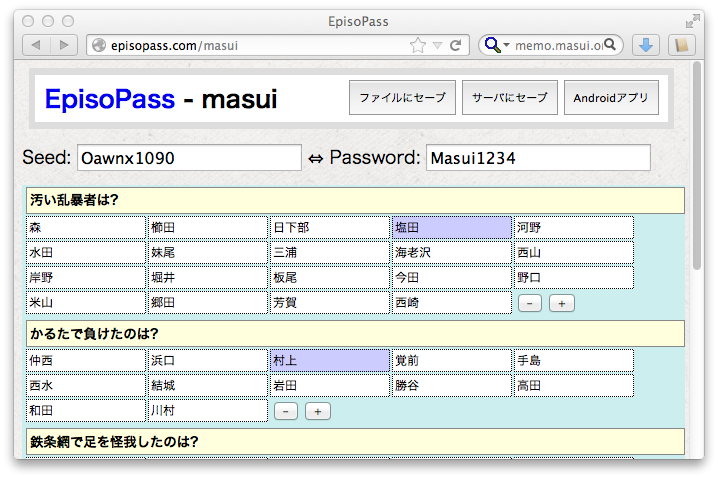
\includegraphics[width=83mm,bb=0 0 718 479]{figures/fab9c55242e1d52c89ff1b46d77b3168.png}}
\caption{既存の{\PW}を利用.}
\label{web4}
\end{figure}

{\PW}以外の秘密の文字列も管理することができる。
たとえば自転車の鍵番号「\textsf{1234}」を{\EP}で管理したい場合、
「\textsf{jitensha-0000}」という{\SS}を入力した後で
{\PW}枠の数字を「\textsf{1234}」に変更することにより、
図\ref{web5}のように「\textsf{jitensha-6145}」という{\SS}で
鍵番号を管理できるようになる。

\begin{figure}[H]
\centerline{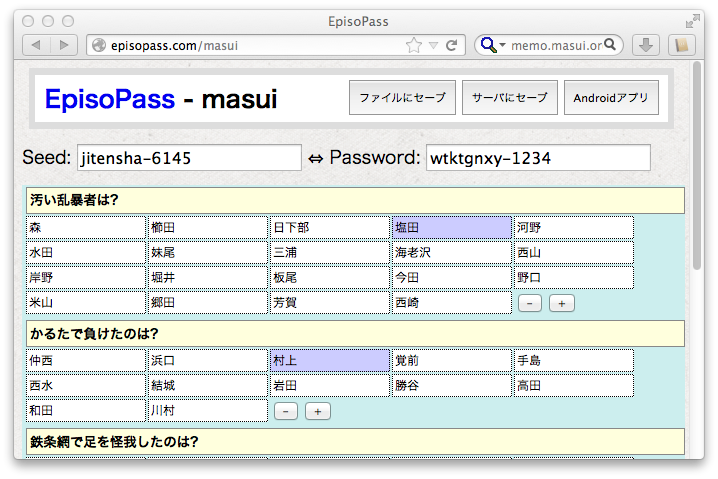
\includegraphics[width=83mm,bb=0 0 718 479]{figures/494cef6da1be0a069ee56e7ec8dcb9a7.png}}
\caption{既存の{\PW}を利用.}
\label{web5}
\end{figure}

既存の{\PW}管理システムは、
利用中の{\PW}を記憶するもの%
\cite{OnePassword}%
\cite{Dashlane}%
\cite{ミルパス}%
\cite{LastPass}%
\cite{KeyPass}%
\cite{NortonIDSafe}%
\cite{IDManager}%
と新しい{\PW}を生成するもの%
\cite{SuperGenPass}%
に分類されるが、
{\EP}はこの両方をサポートしている。

\subsubsection{Androidアプリ}

Webサービスを利用する場合、ブラウザとサーバとの間の通信を
記録されたり盗み見されたりされる心配を完全に払拭することはできない。
% 危険を完全になくすことはできない。
前述の例において、
{\PW}はブラウザ内部でJavaScriptにより生成されるので、
一度ページを表示した後は
ネットワークを遮断しても{\PW}計算を行なえるようになっているが、
最初から全く通信を行なわずに{\PW}を作成できる方がより安心であろう。
このため、通信を全く行なわずにマシン単体で{\PW}計算を行なうための
Androidアプリを用意した。
ページの右上の「Androidアプリ」ボタンを押すと、
現在表示している秘密の問題と答を内蔵したAndroidアプリが
サーバ上でビルドされてダウンロードされる。

Android端末でアプリを実行すると図\ref{android1}のような画面が表示される。
{\SS}を設定して「開始」ボタンを押すと図\ref{android2}のように質問がひとつずつ表示され、
ボタンを押してすべて回答すると{\PW}が計算され図\ref{android3}のように表示される。

\begin{figure}[H]
\centerline{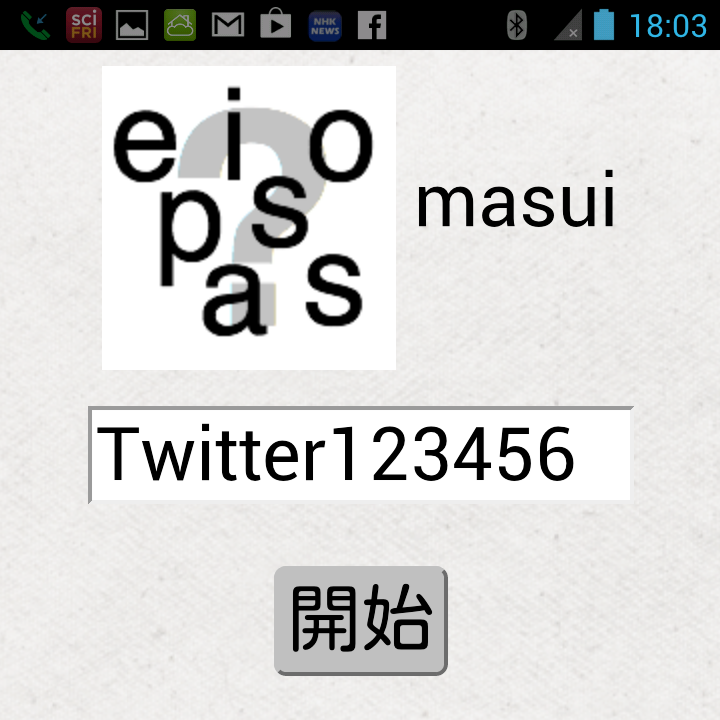
\includegraphics[width=50mm,bb=0 0 720 720]{figures/android1crop.png}}
\caption{Androidアプリ初期画面.}
\label{android1}
\end{figure}

\begin{figure}[H]
\centerline{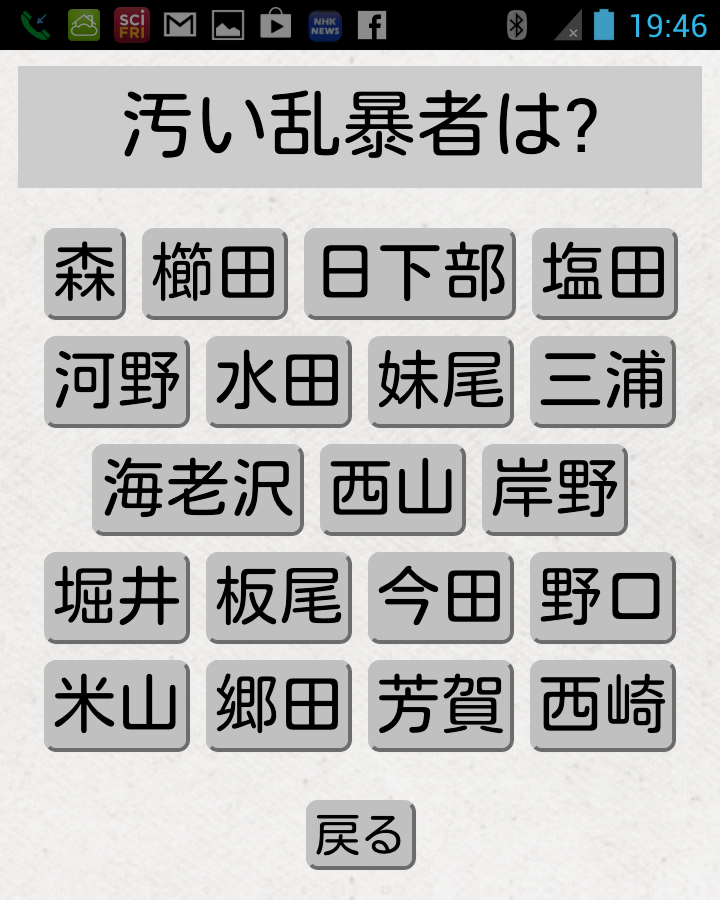
\includegraphics[width=50mm,bb=0 0 720 900]{figures/android2crop.png}}
\caption{最初の問題.}
\label{android2}
\end{figure}

\begin{figure}[H]
\centerline{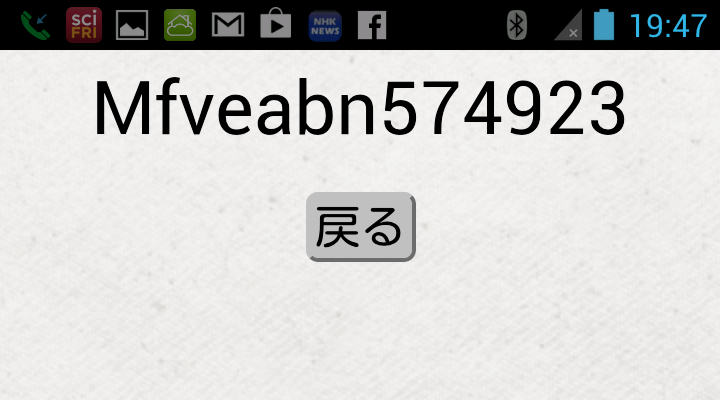
\includegraphics[width=50mm,bb=0 0 720 400]{figures/android3crop.png}}
\caption{すべての問題に回答した後の状態.}
\label{android3}
\end{figure}

回答入力と{\PW}計算はAndroid端末で実行されるため、
端末を「機内モード」に設定するなどの方法で
ネットワーク接続を遮断した状態でも{\PW}を計算することができる。
{\EP}をインストールしたAndroid端末を持っていれば常に各種の{\PW}を計算できるので、
他人のマシンや公共の場所に設置されたパソコンなどでも
容易にtwitterなどのネットサービスを利用することができる。

前述の方法で{\EP}アプリをサーバからダウンロードする場合は、
ブラウザ上で秘密の問題をサーバに登録する必要があるが、
秘密の問題を全くネット上に露出することなくアプリを利用することもできる。
秘密の問題を含まない{\EP}アプリをGoogle Playで公開\footnote{
 {\textsf{https://play.google.com/{\allowbreak}store/{\allowbreak}apps/{\allowbreak}details?{\allowbreak}id=com.{\allowbreak}pitecan.{\allowbreak}episo\_pass}}
}しているので、
これを端末にインストールした後、
ローカルマシンで作成した{\SQ}を端末に転送すれば
\textsf{EpisoPass.comから}ダウンロードしたアプリと同様に利用できる。
この手法を使うと{\SQ}が通信路を通ることがないので安全であるが、
アプリのセットアップの手間は増える。

\subsection{{\PW}文字列の計算方法}

問題と回答から文字列を生成し、そのMD5値によって{\SS}を換字することにより
{\PW}を生成している。
{\PW}文字列の計算方法は附録に示す。

\section{議論}

{\EP}の利便性、安全性、運用の問題などについて考察する。

\subsection{運用形態と安全性}

{\PW}管理システムにおいて最も重要なのは安全性である。
%
{\EP}は様々な運用方法が可能であり、
運用形態によって安全性の評価が異なるので、
利用例にもとづいて{\EP}の安全性を考える。

\subsubsection{\protect{\textsf{\EP}}の利用を秘密にする場合}
\label{pattern1}

{\PW}管理に{\EP}を利用していることを公開せず、
単なる{\PW}生成機として利用する場合は、
普通に{\PW}を利用する場合に比べて安全度が低下することは無い。
{\PW}として充分強力な文字列を{\SS}として利用すれば
{\EP}によって換字された文字列も{\PW}として強力だと考えられるし、
推測しやすい文字列を{\SS}として設定した場合であっても
ランダムな換字操作によってより強力な{\PW}が生成されるので、
{\EP}を利用するデメリットは無く、
通常の{\PW}管理システムと同様の方法で利用できる。

\subsubsection{{\SS}を秘密にする場合}
\label{pattern2}

{\EP}の{\SQ}を公開した場合でも、
{\SS}を通常の{\PW}と同じレベルで秘密にしておけば
SuperGenPass\cite{SuperGenPass}と同じレベルの利便性と安全性が確保できる。
\ref{pwgen}で述べた方法を利用することにより、
ひとつの{\SS}から複数の{\PW}を生成することができる。

\subsubsection{すべて公開する場合}
\label{pattern3}

{\SQ}を解くことが不可能であれば、
{\SS}と{\SQ}をすべて公開しても安全である。
この場合、
ユーザは{\SQ}と{\SS}を通常のテキストデータと同じように管理できるし、
{\PW}管理のために新しく記憶しなければならない情報が皆無なので、
ユーザは{\PW}管理について注意を払う必要が無くなり気が楽になる。

{\SQ}を解くことを困難にするためには質問の数と偽答の数が多くなければならないし、
自分だけが知っている{\EM}をうまく{\SQ}にするにはコツが必要である。
良い{\SQ}を作る方法に関しては\ref{goodquestions}で議論するが、
すべての質問を公開するのが心配な場合や、
{\SQ}の数や質がが充分でないと感じられる場合は
\ref{pattern1}や\ref{pattern2}の手法で運用し、
徐々に運用方法を変えていけば良いだろう。

\subsection{{\SQ}の強度}

% 選択式のとそうでないものと

% すべての計算結果を他人に見せなければ総当たり攻撃は回避できる。

{\PW}は長年利用されているため
強度や実際の運用に関して多くの研究が存在するが%
\cite{Hayashi:2011:DSP:1978942.1979326}%
\cite{Komanduri:2011:PPM:1978942.1979321}% どういうパスワードが強いか
、{\SQ}の強度に関しては充分研究されていない。
{\EP}の運用実績は長くないが安全性などについて考察を行なう。

{\EP}で
選択枝が10個の{\SQ}を8個使用する場合、
総当たりで{\PW}を生成するには
1億($10^8$)通りの試行が必要であり、
% エントロピーは26.6 ($ = 8 \times \log_2 10$) ビット
エントロピーは26.6ビットとなる。
英字からランダムに8文字を並べて作成した{\PW}のエントロピーは37.6ビットになるが、
``\textsf{pmvixuzq}''のように全く意味のない{\PW}を記憶して利用することは少ないため、
実際に利用される{\PW}のエントロピーは20ビット程度と考えられているので\cite{NIST}、
{\SQ}と選択枝の数を10個程度用意すれば
通常の{\PW}と同程度の強度が期待できることになる。
%
総当たり攻撃が可能なオフライン運用ではエントロピーの大きさは重要であるが、
オンラインサービスでは
{\PW}入力を何度か間違えるとサービスがブロックされるのが普通なので、
それほど長い{\PW}を用意する必要は無いと考えられている\cite{Florencio:2007:SWP:1361419.1361429}。

一方、{\SQ}を利用する認証の脆弱性を利用した攻撃が近年問題になっている。
{\PW}を忘れたときのために、
あらかじめ設定した{\SQ}に答えることによって{\PW}をリセットできるサービスがあり、
「母親の旧姓は?」や「最初に飼ったペットの名前は?」のような
質問に対してユーザが答を登録するようになっている。
このような問題は他人が調べたり推測したりすることが容易であるうえに
{\SQ}の数は一般的に少なく、
{\PW}よりも脆弱だといえる\cite{Rabkin:2008:PKQ:1408664.1408667}。% 銀行20個調べて{\SQ}の弱さを指摘
%
ユーザが作成した{\SQ}を使えばこのような問題はなくなるはずであるが、
他人に解かれにくい問題をユーザが作成することは難しく、
またユーザ自身が答を忘れてしまうことも多いと考えられている\cite{Just:2009:PCC:1572532.1572543}\cite{Schechter:2009:NSM:1607723.1608145}。
%
また、古い記憶にもとづいて作成した秘密の問題は
ユーザが想像するよりも解かれやすいという実験結果にもとづき、
忘れない{\SQ}を複数利用する方法、
問題と答を連想するために画像を利用する方法、
複数の問題を連続的に利用する手法などが提案されている\cite{Renaud:2010:PQE:2146303.2146318}。

{\EP}では、
他人には解くことが難しく自分では忘れないような{\SQ}を自由にいくつでも利用できるようになっている。
問題作成に慣れていないユーザには有効な{\SQ}を作成することは難しいかもしれないが、
次節で述べるように、適切な質問を選ぶことによりこの問題を解決できるはずである。

\subsection{{\SQ}の選択}
\label{goodquestions}

{\EP}利用において{\SQ}の選択は非常に重要である。
他人が推測することが難しく、自分が決して忘れないような{\EM}を{\SQ}として利用すべきであり、
以下のような性質をもつ記憶は{\SQ}として利用すべきではない。

\begin{itemize}
\item \textsf{自慢になるもの
(何かの機会にうっかり他人に話してしまう可能性がある)}

\vspace{-1mm}
\item \textsf{ネット上に記録が残っているもの}

\vspace{-1mm}
\item \textsf{他人と情報を共有しているもの}

\vspace{-1mm}
\item \textsf{趣味や嗜好に関連するもの
(他人に推測されやすいうえに嗜好が変化する可能性がある)}

\end{itemize}

\noindent
このようなものではなく、
「わざわざ人に話すことはないが自分の記憶に強く残っているような無難な{\EM}」を
{\SQ}として利用するのが良いであろう。
具体例としては以下のようなものがある。

\begin{itemize}
\item 昔のちょっとした怪我の場所や種類

\vspace{-1mm}
\item 昔のちょっと悔しい思い出

\vspace{-1mm}
\item 昔何かを見つけた場所
\end{itemize}

たとえば図\ref{kega}のような{\SQ}は他人に話したことが無いが、
痛い思いをしたことは忘れないし、
偽答を作成するのも簡単なので、
認証のための{\SQ}として適切であると考えられる。

\begin{figure}[H]
\centerline{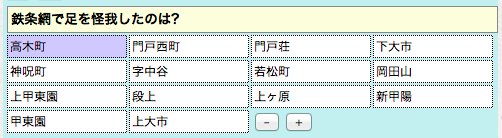
\includegraphics[width=83mm,bb=0 0 502 138]{figures/5c50eed4646232e070646f87b2c8565c.png}}
\caption{昔の怪我に関する{\SQ}.}
\label{kega}
\end{figure}

% 学生に作ってもらった例
%   みんなで行った店は
%   好きな言葉は
% 
% デルタの柵の上にあるのは?
% 
% Autobiographical Authenticationは全然駄目だという\cite{林}
% そんなものすぐ忘れる

\subsection{偽答の作成方法}

{\SQ}の種類によっては偽答の生成が難しい場合がある。
図\ref{atmega}は電子工作に関する{\SQ}の例であるが、
正答と区別がつかない偽答を充分リストすることは難しい。

\begin{figure}[H]
\centerline{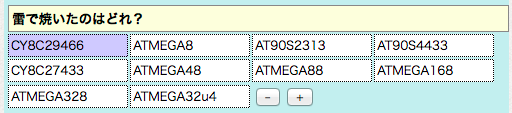
\includegraphics[width=83mm,bb=0 0 512 113]{figures/2f63ceb9ab6faf8d81393953f2f95a8c.png}}
\caption{偽答の生成が難しい例.}
\label{atmega}
\end{figure}

一方、正答として人名や地名を利用する場合、
正答に似た人名や地名をリストすることは難しくない。
「世田谷」が正答であるとき、
「目黒」「杉並」のような偽答を用意するのは簡単である。
%
正答と同じカテゴリに属する単語を自動的にリストすることができれば
正答をもとにして簡単に偽答のリストを生成することができる。
%
ひとつの単語もしくは単語の集合と同じカテゴリに属する単語を検索する手法は
「同位語検索」と呼ばれ、
Webのデータを利用した様々な同位語検索システムが提案されている%
\cite{Huang:2012:LFC:2426725.2426728}% 読んでないけど
\cite{BooWa}% Boo!Wa!というサイトをやっている
\cite{Wang:2007:LSE:1441428.1442086}% BooWa
\cite{大島裕明:2006-12-15}% ライバルサーチ「やーやら」
。
たとえば「ライバルサーチ『やーやら』」\cite{大島裕明:2006-12-15}は、
Web上の「AやBが」のような表現を抽出することによって
AとBのカテゴリが近いことを判断している。

人名や地名の偽答を作成したい場合は
人名や地名のデータベースを利用して偽答を生成することができる。
市町村の人口ランキングや位置関係のデータなどを利用すれば
似た地名を偽答としてリストすることが可能であるし、
人名ランキングを利用すれば
似た苗字を偽答とすることができる。
たとえば日本の名字ランキングの40位近辺に
「長谷川」「近藤」「石井」「斉藤」「坂本」「遠藤」「藤井」
などの名字があるので、
「石井」が正答のときこれらの名字を偽答にすればよい。
しかし、
「小学生のとき〜だった同級生は誰?」という{\SQ}の正答が「石井」であるとき
この方法で偽答を生成すると、
「長谷川」「近藤」などの同級生の存在を確認することにより
正答が「石井」であることが判明してしまう可能性があるので注意が必要である。

% こういう危険は沢山存在するし、
% ソーシャルエンジニアリング\cite{ソーシャル}にひっかかる可能性も高いから
% 完全に安全なものは難しいかもしれない

%原理は簡単で、ソースを全公開しているので問題があれば指摘されることが期待できる
%
\subsection{{\PW}漏洩時の問題}

{\SQ}を公開している場合、
{\SS}と{\PW}の対応がひとつでも漏洩してしまうと、
総当たり計算でチェックすることにより、
すべて{\SQ}の正答が判明してしまう。
{\SQ}の正答を知っていれば
{\SS}から{\PW}を計算することができるので、
漏洩した{\SQ}は利用不可能になってしまう。
%
\ref{pattern1}や
\ref{pattern2}のような運用をしている場合は
{\PW}がひとつ漏洩しても他の{\PW}は安全だが、
\ref{pattern3}のような運用をしている場合は
ひとつでも{\PW}が漏洩するとあらゆる{\PW}が漏洩してしまうことになる。

通常のWebサービスなどの{\PW}が漏洩することは考えにくいが、
「自転車の鍵番号」のように
家族などで共有する可能性があるものに対して
\ref{pattern3}のような運用を行なうと、
鍵番号を知っている人物が総当たり攻撃を行なうことによって
{\SQ}の答が判明してしまう。
% \ref{pattern3}のように
{\SS}や{\SQ}を秘密情報として扱わない場合は
{\PW}を他人と共有しないように注意する必要がある。

\subsection{正答の指定手法について}

{\EP}では{\SQ}の答をリストから選択する方法をとっているが、
{\SQ}によって{\PW}を回復できるWebサービスなどでは
ユーザが回答文字列を入力する方法をとっているものが多い。
リストから答を選択するよりも文字列を入力する方がより安全と思われるが、
文字端末でのコマンド入力がGUIのメニュー操作より難しいのと同様に、
入力するテキストを忘れたり間違えたりする可能性が高くなってしまうというデメリットがある。
「日本の首都は?」のような簡単な質問であっても
「東京」「Tokyo」「tokyo」「toukyou」のどれが正解か迷うかもしれない。
自由なテキスト入力を行なうよりも、
選択式の回答を多数提示して選択させる方が高速に誤りのない操作が可能であり、
利便性が高く充分安全な運用が可能である。

% \subsection{{\EM}をいろんなものに変換する面白さ}
% 
% {\PW}に限らないだろう
% 
% 指紋を{\PW}に変換することなども考えられる
% 
% 指紋はコピーされる
% 
% 脳はコピーされない
% 
% 同じ考え方は通用するだろう

\subsection{画像認証の利用}

忘れにくい{\EM}を利用する認証手法として
様々な画像認証システム\cite{Biddle:2012:GPL:2333112.2333114}\cite{GraphicalPasswords}\cite{小池英樹:2006-05-15}が提案されている。
複数の画像の中から正答を選択するもの(Cognometric方式)、
ひとつの画像の中の特定の場所を指定するもの(Locimetric方式)、
画像の上で描画操作を行なうもの(Drawmetric方式)
が広く利用されているが\cite{Biddle:2012:GPL:2333112.2333114}\cite{GraphicalPasswords}\cite{Guideline}、
{\EP}は図\ref{web1}のように
文字列のかわりに画像URLを{\SQ}として利用する点が異なっている。
%
Cognometric方式は{\EM}を効果的に利用できるが、
多数の偽答画像が必要だという問題がある。
Locimetric方式は
{\EM}を効果的に利用できないことに加え、
クリックしやすい「ホットスポット」は限られているため
充分なエントロピーを確保できないことが問題になる\cite{Dirik:2007:MUC:1280680.1280684}。
またDrawmetric方式も{\EM}を効果的に利用できないし、
ユーザは似た傾向のストロークを選びがちであるため
充分なエントロピーを確保しにくいことが知られている\cite{Nali}。
%
{\EP}のように画像を{\SQ}として利用する場合、
通常の{\SQ}の場合と同様に偽答を増やすことが容易であることに加え、
画像に関連した{\EM}を有効に利用できるという利点がある\cite{増井:CSS}。

図\ref{leiko}は
本棚.org\cite{hondana}\cite{hondanaorg}
のユーザのひとり\footnote{
  \textsf{http://hondana.org/Leiko}
}が利用している画像認証問題である。
このユーザ以外には正答は見当もつかないが、
本人にとっては忘れることがない{\EM}と結びついた画像だということであった。

\begin{figure}[H]
% \centerline{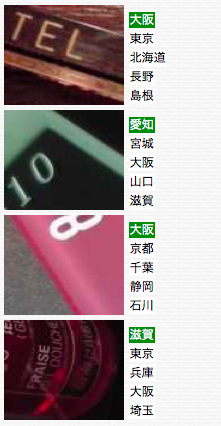
\includegraphics[width=40mm,bb=0 0 221 426]{figures/5a26c3b31834ddeb04edf4593b891647.png}}
\centerline{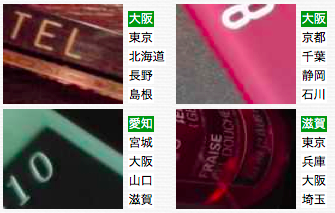
\includegraphics[width=75mm,bb=0 0 335 213]{figures/4084ac59b42d183d7124481477e84999.png}}
\caption{{\EM}と深く結びついた画像.}
\label{leiko}
\end{figure}

%\subsection{安心感の問題} 
%
%心配に感じる点
% => 単純な問題の場合、自分が知ってることは他人も知ってそうに思える
%
%知ってる話ばかりだと心配になる

%\subsection{変わった応用}
%
%家族でパスワードをシェア
%
%WiFiのパスワードを学会でシェアするとか

\section{結論}

{\EM}に結びついた{\SQ}を利用して{\PW}を生成/管理できるシステム{\EP}を提案した。
{\EP}は単純な原理にもとづいており柔軟な利用形態が可能であり、
強力な{\SQ}を用意することにより
秘密情報を全く覚えることなく安全な認証を行なうことができる。
%
強力な{\SQ}を作成して安全に運用が可能かどうかを長期的に評価したいと考えている。
%
%欠点:
%なぞなぞを考えるのがめんどくさい
%安全になぞなぞを扱うのが面倒
%  ネットなしで運用したりとか
%運用を間違うと思わぬところで回答がバレる可能性がある
%
{\EP}は\textsf{http://Episopass.com/}で運用しており、
ソースはGitHubで公開している\footnote{
  \textsf{http://GitHub.com/masui/EpisoPass}
}。

{\scriptsize
\bibliographystyle{jwiss}
\bibliography{paper}
}

\section*{附録: {\PW}計算アルゴリズム}

{\PW}は、
{\SQ}と回答の組合せにもとづいて{\SS}を換字することによって計算される。
換字は文字種ごとに行なわれる。
たとえば
{\SS}の1桁目が数字のときは{\PW}の1桁目は数字に変換され、
{\SS}の1桁目が記号のときは{\PW}の1桁目は記号に変換される。

{\SS}内の数字$A$は、換字関数$f_N()$によって{\PW}内の数字$B$に変換される。
$f_N()$ は以下のような関数である。

\[ f_N(x) = (10 + N - x) \bmod 10 \]

ここで$N$は{\SS}と回答の組み合わせから計算される自然数で、
答の選択により変化する。
たとえば$N = 5$ のとき、$f_5(x) = (15-x) \bmod 10$ となるので、
$x$と$f_5(x)$の対応は以下のようになる。

\[ f_5(0) = 5 \]
\[ f_5(1) = 4 \]
\[ f_5(2) = 3 \]
\[ ... \]
\[ f_5(8) = 7 \]
\[ f_5(9) = 6 \]

$f_N()$は$N$により変化するので、$N$がわからなければ$f_N()$もわからない。
$N$は{\SS}と回答の組み合わせから計算される自然数なので、
{\SS}の答を知らなければ$N$を計算することはできず、
問題と答の組み合わせを知らない限り{\SS}から{\PW}を計算することはできない。

{\EP}では以下のようにして$f_N()$を計算している。

\begin{enumerate}
\item 問題文字列と選択した答の文字列の組を連結して長い文字列$S$を生成

\vspace{-1mm}
\item $S$のMD5ハッシュ値$M$(16進32桁の文字列)を計算

\vspace{-1mm}
\item {\SS}の$k$桁目の文字に対し、
$M$の$k \times 4$文字目から$k \times 4 + 3$文字目までの部分文字列(16進4桁)を取得し、
それを$N$とする

たとえばハッシュ値$M$が$12345678...$だったとき、1桁目を計算する$f()$についてはN=0x1234となる。
\end{enumerate}

\end{document}
